\documentclass[]{article}
\usepackage{lmodern}
\usepackage{amssymb,amsmath}
\usepackage{ifxetex,ifluatex}
\usepackage{fixltx2e} % provides \textsubscript
\ifnum 0\ifxetex 1\fi\ifluatex 1\fi=0 % if pdftex
  \usepackage[T1]{fontenc}
  \usepackage[utf8]{inputenc}
\else % if luatex or xelatex
  \ifxetex
    \usepackage{mathspec}
  \else
    \usepackage{fontspec}
  \fi
  \defaultfontfeatures{Ligatures=TeX,Scale=MatchLowercase}
\fi
% use upquote if available, for straight quotes in verbatim environments
\IfFileExists{upquote.sty}{\usepackage{upquote}}{}
% use microtype if available
\IfFileExists{microtype.sty}{%
\usepackage{microtype}
\UseMicrotypeSet[protrusion]{basicmath} % disable protrusion for tt fonts
}{}
\usepackage[margin=1in]{geometry}
\usepackage{hyperref}
\hypersetup{unicode=true,
            pdftitle={Trabalho de dados Binários},
            pdfauthor={Laís Hoffmann, Simone Matsubara, Yasmin Fernandes, Willian Meira},
            pdfborder={0 0 0},
            breaklinks=true}
\urlstyle{same}  % don't use monospace font for urls
\usepackage{color}
\usepackage{fancyvrb}
\newcommand{\VerbBar}{|}
\newcommand{\VERB}{\Verb[commandchars=\\\{\}]}
\DefineVerbatimEnvironment{Highlighting}{Verbatim}{commandchars=\\\{\}}
% Add ',fontsize=\small' for more characters per line
\usepackage{framed}
\definecolor{shadecolor}{RGB}{248,248,248}
\newenvironment{Shaded}{\begin{snugshade}}{\end{snugshade}}
\newcommand{\KeywordTok}[1]{\textcolor[rgb]{0.13,0.29,0.53}{\textbf{{#1}}}}
\newcommand{\DataTypeTok}[1]{\textcolor[rgb]{0.13,0.29,0.53}{{#1}}}
\newcommand{\DecValTok}[1]{\textcolor[rgb]{0.00,0.00,0.81}{{#1}}}
\newcommand{\BaseNTok}[1]{\textcolor[rgb]{0.00,0.00,0.81}{{#1}}}
\newcommand{\FloatTok}[1]{\textcolor[rgb]{0.00,0.00,0.81}{{#1}}}
\newcommand{\ConstantTok}[1]{\textcolor[rgb]{0.00,0.00,0.00}{{#1}}}
\newcommand{\CharTok}[1]{\textcolor[rgb]{0.31,0.60,0.02}{{#1}}}
\newcommand{\SpecialCharTok}[1]{\textcolor[rgb]{0.00,0.00,0.00}{{#1}}}
\newcommand{\StringTok}[1]{\textcolor[rgb]{0.31,0.60,0.02}{{#1}}}
\newcommand{\VerbatimStringTok}[1]{\textcolor[rgb]{0.31,0.60,0.02}{{#1}}}
\newcommand{\SpecialStringTok}[1]{\textcolor[rgb]{0.31,0.60,0.02}{{#1}}}
\newcommand{\ImportTok}[1]{{#1}}
\newcommand{\CommentTok}[1]{\textcolor[rgb]{0.56,0.35,0.01}{\textit{{#1}}}}
\newcommand{\DocumentationTok}[1]{\textcolor[rgb]{0.56,0.35,0.01}{\textbf{\textit{{#1}}}}}
\newcommand{\AnnotationTok}[1]{\textcolor[rgb]{0.56,0.35,0.01}{\textbf{\textit{{#1}}}}}
\newcommand{\CommentVarTok}[1]{\textcolor[rgb]{0.56,0.35,0.01}{\textbf{\textit{{#1}}}}}
\newcommand{\OtherTok}[1]{\textcolor[rgb]{0.56,0.35,0.01}{{#1}}}
\newcommand{\FunctionTok}[1]{\textcolor[rgb]{0.00,0.00,0.00}{{#1}}}
\newcommand{\VariableTok}[1]{\textcolor[rgb]{0.00,0.00,0.00}{{#1}}}
\newcommand{\ControlFlowTok}[1]{\textcolor[rgb]{0.13,0.29,0.53}{\textbf{{#1}}}}
\newcommand{\OperatorTok}[1]{\textcolor[rgb]{0.81,0.36,0.00}{\textbf{{#1}}}}
\newcommand{\BuiltInTok}[1]{{#1}}
\newcommand{\ExtensionTok}[1]{{#1}}
\newcommand{\PreprocessorTok}[1]{\textcolor[rgb]{0.56,0.35,0.01}{\textit{{#1}}}}
\newcommand{\AttributeTok}[1]{\textcolor[rgb]{0.77,0.63,0.00}{{#1}}}
\newcommand{\RegionMarkerTok}[1]{{#1}}
\newcommand{\InformationTok}[1]{\textcolor[rgb]{0.56,0.35,0.01}{\textbf{\textit{{#1}}}}}
\newcommand{\WarningTok}[1]{\textcolor[rgb]{0.56,0.35,0.01}{\textbf{\textit{{#1}}}}}
\newcommand{\AlertTok}[1]{\textcolor[rgb]{0.94,0.16,0.16}{{#1}}}
\newcommand{\ErrorTok}[1]{\textcolor[rgb]{0.64,0.00,0.00}{\textbf{{#1}}}}
\newcommand{\NormalTok}[1]{{#1}}
\usepackage{graphicx,grffile}
\makeatletter
\def\maxwidth{\ifdim\Gin@nat@width>\linewidth\linewidth\else\Gin@nat@width\fi}
\def\maxheight{\ifdim\Gin@nat@height>\textheight\textheight\else\Gin@nat@height\fi}
\makeatother
% Scale images if necessary, so that they will not overflow the page
% margins by default, and it is still possible to overwrite the defaults
% using explicit options in \includegraphics[width, height, ...]{}
\setkeys{Gin}{width=\maxwidth,height=\maxheight,keepaspectratio}
\IfFileExists{parskip.sty}{%
\usepackage{parskip}
}{% else
\setlength{\parindent}{0pt}
\setlength{\parskip}{6pt plus 2pt minus 1pt}
}
\setlength{\emergencystretch}{3em}  % prevent overfull lines
\providecommand{\tightlist}{%
  \setlength{\itemsep}{0pt}\setlength{\parskip}{0pt}}
\setcounter{secnumdepth}{0}
% Redefines (sub)paragraphs to behave more like sections
\ifx\paragraph\undefined\else
\let\oldparagraph\paragraph
\renewcommand{\paragraph}[1]{\oldparagraph{#1}\mbox{}}
\fi
\ifx\subparagraph\undefined\else
\let\oldsubparagraph\subparagraph
\renewcommand{\subparagraph}[1]{\oldsubparagraph{#1}\mbox{}}
\fi

%%% Use protect on footnotes to avoid problems with footnotes in titles
\let\rmarkdownfootnote\footnote%
\def\footnote{\protect\rmarkdownfootnote}

%%% Change title format to be more compact
\usepackage{titling}

% Create subtitle command for use in maketitle
\newcommand{\subtitle}[1]{
  \posttitle{
    \begin{center}\large#1\end{center}
    }
}

\setlength{\droptitle}{-2em}

  \title{Trabalho de dados Binários}
    \pretitle{\vspace{\droptitle}\centering\huge}
  \posttitle{\par}
  \subtitle{Acidentes de carro}
  \author{Laís Hoffmann, Simone Matsubara, Yasmin Fernandes, Willian Meira}
    \preauthor{\centering\large\emph}
  \postauthor{\par}
      \predate{\centering\large\emph}
  \postdate{\par}
    \date{2018-11-10}

\usepackage[brazil]{babel} \usepackage{amsmath} \usepackage{float}
\usepackage{bm}

\begin{document}
\maketitle

\section{1. Base de Dados}\label{base-de-dados}

\textbf{1.1 Descrição dos dados}

Os dados foram retirados do pacote ``DAAG'', sendo dados dos EUA, entre
1997-2002, de acidentes de carro relatados pela polícia nos quais há um
evento prejudicial (pessoas ou propriedade) e do qual pelo menos um
veículo foi rebocado. Os dados são restritos aos ocupantes do banco da
frente, incluem apenas um subconjunto das variáveis registradas e são
restritos de outras maneiras também.

A base original possui uma base de dados com 26.217 observações nas 15
variáveis a seguir.

1 - \textbf{veloc}: velocidades estimadas do impacto do acidente:
1-9km/h, 10-24, 25-39, 40-54, 55+ \newline 2 - \textbf{pesos}: Pesos de
observação \newline 3 - \textbf{sobrev}: Classificação se sobreviveu ao
acidente: 1 = morreu ou 0 = sobreviveu \newline 4 - \textbf{airbag}: Se
o carro possui airbag: com ou sem airbag \newline 5 - \textbf{cinto}:
uso do cinto de segurança: com ou sem cinto \newline 6 -
\textbf{frontal}: impacto do acidente: 0 = não frontal, 1 = impacto
frontal \newline 7 - \textbf{sexo}: Sexo: 0 = Feminino ou 1 = Masculino
\newline 8 - \textbf{idade}: Idade dos ocupantes do veículo \newline 9 -
\textbf{anoaci}: Ano do acidente (1997-2002) \newline 10 -
\textbf{anovei}: Ano do veículo (1953-2003) \newline 11 -
\textbf{airbagcat}: Se Airbags foram acionados: deploy, nodeploy,
unavail \newline 12 - \textbf{ocupantes}: Posição do airbag acionado:
driver, pass \newline 13 - \textbf{abfunc}: Airbag acionados: 0: Se não
possuia airbag ou não foi acionado, 1: Um ou mais airbags foram
acionados \newline 14 - \textbf{grav}: Gravidade do acidente: 0:none, 1
= Possível Lesão, 2:no incapacity, 3:incapacity, 4:killed; 5:unknown,
6:prior death \newline 15 - \textbf{numcaso}: Número do caso.

No entanto, escolhemos analisar os dados do ano do acidente de 2002 e
veículos de ano 2000 e retirar as variaveis weight, abcat e caseid.

\section{2 Análise Descritiva}\label{analise-descritiva}

\textbf{2.1 Medidas de Resumo}

\begin{Shaded}
\begin{Highlighting}[]
\KeywordTok{summary}\NormalTok{(dados[ , }\KeywordTok{c}\NormalTok{(}\DecValTok{1}\NormalTok{:}\DecValTok{8}\NormalTok{,}\DecValTok{10}\NormalTok{)])}
\end{Highlighting}
\end{Shaded}

\begin{verbatim}
##        veloc     sobrev    airbag    cinto     frontal     sexo    
##  01-09 mph: 12   Não: 23   Não:  1   Não:121   Não:183   Fem :254  
##  10-24 mph:293   Sim:470   Sim:492   Sim:372   Sim:310   Masc:239  
##  25-39 mph:121                                                     
##  40-54 mph: 46                                                     
##  55+ mph  : 21                                                     
##                                                                    
##                                                                    
##      idade        ocupantes        grav      
##  Min.   :16.00   Driver:386   Min.   :0.000  
##  1st Qu.:23.00   Pass  :107   1st Qu.:0.000  
##  Median :35.00                Median :1.000  
##  Mean   :37.82                Mean   :1.579  
##  3rd Qu.:48.00                3rd Qu.:3.000  
##  Max.   :93.00                Max.   :5.000  
##                               NA's   :4
\end{verbatim}

\textbf{2.3 Histogramas}

\begin{Shaded}
\begin{Highlighting}[]
\KeywordTok{pie}\NormalTok{(}\KeywordTok{table}\NormalTok{(dados$abfunc), }
    \DataTypeTok{main=}\StringTok{"Gráfico de setores: Grau de Instrução"}\NormalTok{) }
\end{Highlighting}
\end{Shaded}

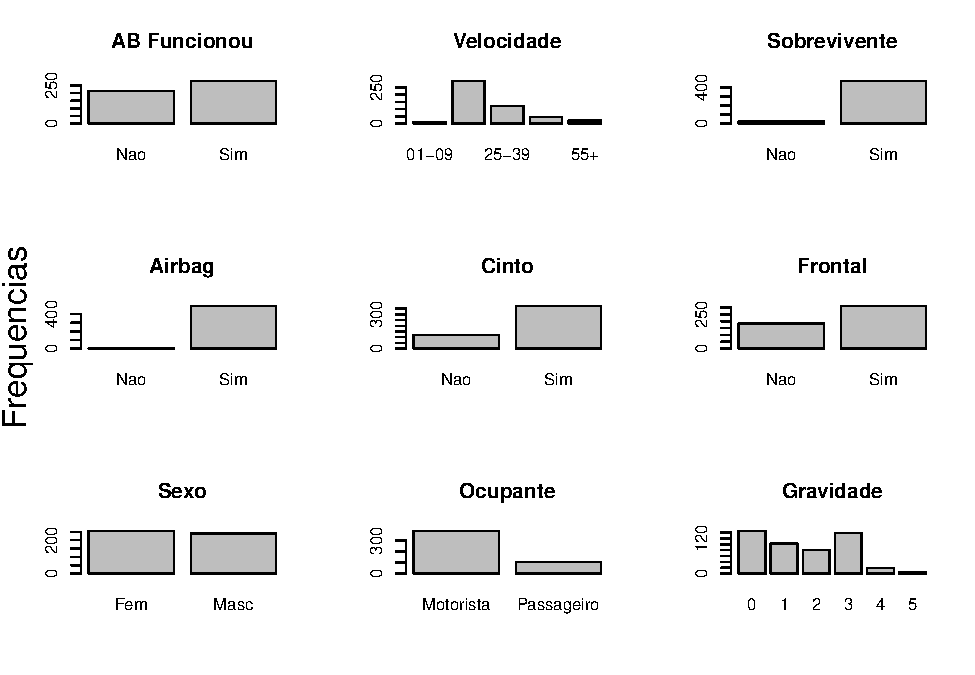
\includegraphics{Dados_Binários1_files/figure-latex/unnamed-chunk-5-1.pdf}

\begin{Shaded}
\begin{Highlighting}[]
\KeywordTok{par}\NormalTok{(}\DataTypeTok{mfrow =} \KeywordTok{c}\NormalTok{(}\DecValTok{3}\NormalTok{,}\DecValTok{3}\NormalTok{))}
\KeywordTok{plot}\NormalTok{(dados$abfunc, }\DataTypeTok{xlab =} \StringTok{''}\NormalTok{, }\DataTypeTok{ylab =} \StringTok{''}\NormalTok{, }\DataTypeTok{main =} \StringTok{'AB Funcionou'}\NormalTok{)}
\KeywordTok{plot}\NormalTok{(dados$veloc, }\DataTypeTok{xlab =} \StringTok{''}\NormalTok{, }\DataTypeTok{ylab =} \StringTok{''}\NormalTok{, }\DataTypeTok{main =} \StringTok{'Velocidade'}\NormalTok{)}
\KeywordTok{plot}\NormalTok{(dados$sobrev, }\DataTypeTok{xlab =} \StringTok{''}\NormalTok{, }\DataTypeTok{ylab =} \StringTok{''}\NormalTok{, }\DataTypeTok{main =} \StringTok{'Sobrevivente'}\NormalTok{)}
\KeywordTok{plot}\NormalTok{(dados$airbag, }\DataTypeTok{xlab =} \StringTok{''}\NormalTok{, }\DataTypeTok{ylab =} \StringTok{''}\NormalTok{, }\DataTypeTok{main =} \StringTok{'Airbag'}\NormalTok{)}
\KeywordTok{plot}\NormalTok{(dados$cinto, }\DataTypeTok{xlab =} \StringTok{''}\NormalTok{, }\DataTypeTok{ylab =} \StringTok{''}\NormalTok{, }\DataTypeTok{main =} \StringTok{'Cinto'}\NormalTok{)}
\KeywordTok{plot}\NormalTok{(dados$frontal, }\DataTypeTok{xlab =} \StringTok{''}\NormalTok{, }\DataTypeTok{ylab =} \StringTok{''}\NormalTok{, }\DataTypeTok{main =} \StringTok{'Frontal'}\NormalTok{)}
\KeywordTok{plot}\NormalTok{(dados$sexo, }\DataTypeTok{xlab =} \StringTok{''}\NormalTok{, }\DataTypeTok{ylab =} \StringTok{''}\NormalTok{, }\DataTypeTok{main =} \StringTok{'Sexo'}\NormalTok{)}
\CommentTok{#plot(dados$idade, xlab = '', ylab = '', main = 'Idade') ### ******* inverteu eixo}
\KeywordTok{plot}\NormalTok{(dados$ocupantes, }\DataTypeTok{xlab =} \StringTok{''}\NormalTok{, }\DataTypeTok{ylab =} \StringTok{''}\NormalTok{, }\DataTypeTok{main =} \StringTok{'Ocupante'}\NormalTok{)}
\KeywordTok{plot}\NormalTok{(dados$grav, }\DataTypeTok{xlab =} \StringTok{''}\NormalTok{, }\DataTypeTok{ylab =} \StringTok{''}\NormalTok{, }\DataTypeTok{main =} \StringTok{'Gravidade'}\NormalTok{)}
\KeywordTok{mtext}\NormalTok{(}\DataTypeTok{side=}\DecValTok{2}\NormalTok{,}\DataTypeTok{cex=}\FloatTok{1.3}\NormalTok{,}\DataTypeTok{line=}\NormalTok{-}\FloatTok{1.5}\NormalTok{,}\DataTypeTok{text=}\StringTok{"Proporção das variaveis"}\NormalTok{,}\DataTypeTok{outer=}\OtherTok{TRUE}\NormalTok{)}
\end{Highlighting}
\end{Shaded}

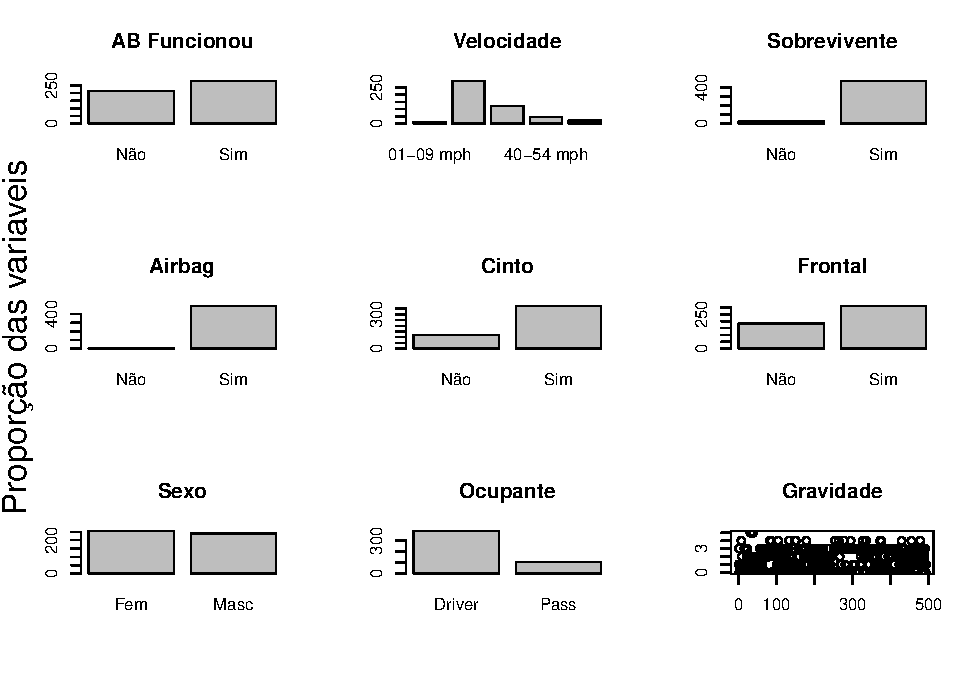
\includegraphics{Dados_Binários1_files/figure-latex/unnamed-chunk-5-2.pdf}

\textbf{2.4 Distribuição}

\textbf{2.5 Análise de correlações entre covariáveis}

\textbf{2.6 Gráficos de Disperção}

\begin{Shaded}
\begin{Highlighting}[]
\NormalTok{a}
\end{Highlighting}
\end{Shaded}

\begin{verbatim}
## NULL
\end{verbatim}

\section{3. AJUSTE DO MODELO DE
REGRESSÃO}\label{ajuste-do-modelo-de-regressao}

\textbf{3.1 Ligação Logito}

\textbf{3.2 Ligação Probito}

\textbf{3.3 Ligação Complemento log-log}

\textbf{3.4 Ligação Cauchy}

\section{4. ESCOLHA DO MODELO}\label{escolha-do-modelo}

\section{5. ANÁLISE DO MODELO AJUSTADO
SELECIONADO}\label{analise-do-modelo-ajustado-selecionado}

\textbf{5.1 Resumo do Modelo}

\textbf{5.2 Reajuste do Modelo}

\textbf{5.3 Análise de Resíduos}

\textbf{5.4 Medidas de Influencia}

\textbf{5.5 Resíduos Quantílicos Aleatoriazados}

\textbf{5.6 Gráfico Normal de Probabilidade com Envelope Simulado}

\textbf{5.7 Gráficos de Efeitos}

\section{6. PREDIÇÃO}\label{predicao}

\section{7. AVALIAÇÃO DO PODER PREDITIVO DO
MODELO}\label{avaliacao-do-poder-preditivo-do-modelo}

\textbf{7.1 Divisão da Base de dados}

\textbf{7.2 Ponto de Corte}

\textbf{7.3 Sensibilidade e Especificidade}

\textbf{7.4 Curva ROC}

\textbf{7.5 Outra Alternativa de validação}

\section{8. REFERÊNCIAS}\label{referencias}

\section{}\label{section}


\end{document}
